\documentclass[journal]{IEEEtran}
% MATUDA --- Multi-Appliance multi-Task Unsupervised Domain Adaptation for NILM
% Journal draft: protocol and method specified for reproducibility; tables marked
% preliminary until multi-seed chronological-split runs complete.

\usepackage{cite}
\usepackage{amsmath,amssymb,amsfonts}
\usepackage{algorithmic}
\usepackage{algorithm}
\usepackage{graphicx}
\usepackage{textcomp}
\usepackage{xcolor}
\usepackage{booktabs}
\usepackage{url}
\usepackage{multirow}
\usepackage{tikz}
\usetikzlibrary{arrows.meta,positioning,fit,calc}
\def\BibTeX{{\rm B\kern-.05em{\sc i\kern-.025em b}\kern-.08em
    T\kern-.1667em\lower.7ex\hbox{E}\kern-.125emX}}

\begin{document}

\title{MATUDA: Multi-Appliance Multi-Task Unsupervised Domain Adaptation for Non-Intrusive Load Monitoring}

\author{\IEEEauthorblockN{Raymond Tie Siou Hin}
\IEEEauthorblockA{\textit{Department of Electrical and Robotics} \\
\textit{Centre for Net-Zero Technology} \\
\textit{Monash University Malaysia} \\
Bandar Sunway, Malaysia}
\and
\IEEEauthorblockN{Tan Wen Shan}
\IEEEauthorblockA{\textit{Department of Electrical and Robotics} \\
\textit{Centre for Net-Zero Technology} \\
\textit{Monash University Malaysia} \\
Bandar Sunway, Malaysia \\
tan.wenshan@monash.edu}
\and
\IEEEauthorblockN{Ding Ze Yang}
\IEEEauthorblockA{\textit{Department of Electrical and Robotics} \\
\textit{Centre for Net-Zero Technology} \\
\textit{Monash University Malaysia} \\
Bandar Sunway, Malaysia}
\and
\IEEEauthorblockN{Mirza Rayana Sanzana}
\IEEEauthorblockA{\textit{School of Information Technology} \\
\textit{Monash University Malaysia} \\
Bandar Sunway, Malaysia}
\and
\IEEEauthorblockN{Haval Kamil}
\IEEEauthorblockA{\textit{Department of Air Conditioning and Refrigeration} \\
\textit{College of Engineering Technology} \\
\textit{Al-Kitab University} \\
Kirkuk, Iraq}
}

\maketitle

\begin{abstract}
Deploying non-intrusive load monitoring (NILM) in a new building requires recognizing multiple appliances simultaneously---both on/off states and power---while typically only the aggregate meter is available at the target site.
Existing unsupervised domain adaptation (UDA) methods for NILM are dominated by single-appliance models; multi-appliance networks are usually transferred with labeled target fine-tuning.
This paper studies unsupervised cross-building transfer of a joint multi-label classification and multi-appliance regression model.
We propose MATUDA, a sequence-to-sequence CNN--temporal convolutional network (TCN) with a shared pointwise fully connected (FC) adaptation tower and $K$ appliance-specific heads.
Domain discrepancy is measured on time-pooled FC activations by a hybrid MMD+CORAL loss, following Deep CORAL, DAN, and late-layer NILM adaptation practice~\cite{sun2016deepcoral,long2015dan,lin2022dda}, and refined by entropy-gated conditional domain alignment (EGC-DA) inspired by conditional adaptation in computer vision~\cite{long2018cdan}.
On UK-DALE (labeled Houses~1+5 $\rightarrow$ unlabeled House~2 aggregates $\rightarrow$ held-out House~2 test), preliminary results show that MATUDA raises target macro-F1 substantially over source-only and global FC-UDA, while relative energy error (SAE) can worsen---a trade-off we report explicitly.
\end{abstract}

\begin{IEEEkeywords}
NILM, multi-appliance, multi-label learning, unsupervised domain adaptation, sequence-to-sequence, TCN, transfer learning
\end{IEEEkeywords}

%======================================================================
\section{Introduction}
%======================================================================
Non-intrusive load monitoring (NILM) estimates appliance-level consumption from a single aggregate meter~\cite{hart1992nilm,kelly2015ukdale}.
Deep sequence models have advanced both power estimation and on/off recognition~\cite{kelly2015neural,zhang2018seq2point}, and multi-appliance architectures jointly decode several loads~\cite{faustine2020unet,xiong2023matnilm}.
In practice, however, a newly instrumented house rarely provides submeter labels.
A model trained on labeled houses must therefore transfer under domain shift induced by occupancy, wiring, and appliance mixes.

Two research lines address only part of this problem.
\textbf{Unsupervised domain adaptation (UDA)} for NILM---MMD/CORAL, adversarial alignment, Sinkhorn hybrids---is mature for \emph{single}-appliance disaggregation~\cite{liu2022uda,lin2022dda,xiong2026ahda,lu2026edge}.
\textbf{Multi-appliance / multi-label} models are usually trained in-domain or transferred by fine-tuning with target labels~\cite{li2023multiobjective,sun2025transfer}.
Semi-supervised multi-label domain adaptation exists for usage recognition without joint power regression under fully unlabeled aggregates~\cite{hur2022ssda}.
Consequently, it remains unclear whether UDA designed for one appliance head still helps a shared multi-head system when the target house provides aggregates only~\cite{muaz2024when}.

\textbf{Research question.}
Can one shared network jointly perform multi-label state detection and multi-appliance power estimation, and transfer to an unlabeled target house by aligning fully connected embeddings---without target submeter labels?

We answer affirmatively under a UK-DALE cross-building protocol in which domain losses are attached to an FC tower (rather than only raw temporal maps) and alignment is entropy-gated and appliance-conditional to limit negative transfer across sparse heads.
Table~\ref{tab:gap} situates the contribution.

\begin{table}[!t]
\caption{Position of this work relative to prior NILM transfer.}
\label{tab:gap}
\centering
\scriptsize
\begin{tabular}{@{}lll@{}}
\toprule
Setting & Supervised / fine-tune & Unsupervised DA \\
\midrule
Single-appliance & \cite{dincecco2020transfer} & \cite{liu2022uda,lin2022dda,lu2026edge} \\
Multi-app.\ (state+power) & \cite{sun2025transfer,li2023multiobjective} & \textbf{this work} \\
Multi-label classification only & \cite{tanoni2023weak} & SSDA~\cite{hur2022ssda} \\
\bottomrule
\end{tabular}
\end{table}

\textbf{Contributions.}
\begin{enumerate}
\item We formulate unsupervised cross-building transfer for joint multi-label classification and multi-appliance regression.
\item We design MATUDA: a sequence-to-sequence CNN--TCN, a shared pointwise FC adaptation tower with multi-layer MMD+CORAL, $K$ appliance-specific heads, and EGC-DA (entropy gate + appliance-conditional alignment).
\item We specify a reproducible UK-DALE protocol (Houses~1+5 labeled $\rightarrow$ House~2 unlabeled adaptation $\rightarrow$ chronologically held-out House~2 test; Houses~3/4 excluded for this appliance set) and compare Source-Only and Global FC-UDA under the same backbone.
\end{enumerate}

%======================================================================
\section{Related Work}
%======================================================================
\subsection{Single-appliance transfer and UDA}
Cross-domain NILM often freezes convolutional layers and retunes dense layers with target labels~\cite{dincecco2020transfer}.
UDA methods align source and target features with MMD/CORAL on late layers~\cite{lin2022dda}, adversarial joint adaptation~\cite{liu2022uda}, hierarchical CORAL+MK-MMD~\cite{xiong2026ahda}, and Sinkhorn+CORAL~\cite{lu2026edge}.
Deep CORAL and DAN establish aligning FC activations in vision~\cite{sun2016deepcoral,long2015dan}; CDAN conditions adversarial alignment on classifier predictions and entropy~\cite{long2018cdan}.
These works motivate FC-layer alignment and conditional / entropy-aware transfer, but assume a single appliance head.

\subsection{Multi-appliance and multi-label NILM}
Multi-task U-Nets and hierarchical multi-appliance networks jointly predict several loads~\cite{faustine2020unet,xiong2023matnilm}.
Cross-house multi-appliance transfer with target labels appears in~\cite{li2023multiobjective,sun2025transfer}.
Hur \emph{et al.} study semi-supervised domain adaptation for multi-label usage recognition~\cite{hur2022ssda}, without unsupervised joint power regression.
Our work keeps the multi-task head design and adds unsupervised FC-layer adaptation with EGC-DA.

%======================================================================
\section{Problem Formulation}
%======================================================================
Let an aggregate active-power window be $x\in\mathbb{R}^{T}$.
For $K$ appliances, let $y\in\mathbb{R}^{T\times K}$ and $z\in\{0,1\}^{T\times K}$ denote the power and on/off trajectories over the same window (sequence-to-sequence supervision).
The \textbf{source domain} $\mathcal{S}$ provides labeled windows $\{(x_S,y_S,z_S)\}$.
The \textbf{target domain} $\mathcal{T}$ provides unlabeled aggregates $\{x_T\}$ during adaptation.
A shared network $f_\Theta$ maps $x$ to predictions $(\hat{y},\hat{z})\in\mathbb{R}^{T\times K}\times\mathbb{R}^{T\times K}$.

\textbf{Transfer scenario (cross-building, unsupervised).}
Train on labeled UK-DALE Houses~1 and~5; adapt using House~2 aggregates without appliance labels; evaluate on House~2 with labels used only for metrics.
This matches a realistic deployment where the new building has a smart meter but no submeters.
Fig.~\ref{fig:scenario} summarizes the data flow.

\begin{figure}[!t]
\centering
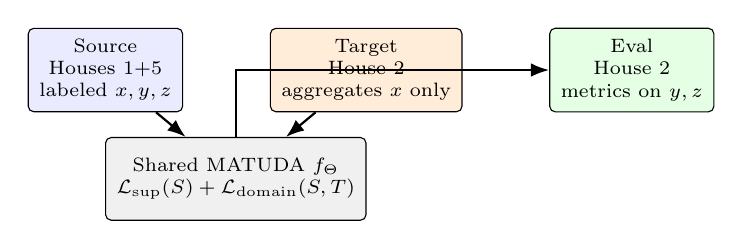
\begin{tikzpicture}[
  font=\scriptsize,
  box/.style={draw, rounded corners=2pt, align=center, inner sep=4pt, minimum height=1.05cm},
  arr/.style={-{Latex}, thick}
]
\node[box, fill=blue!8] (S) {Source\\Houses 1+5\\labeled $x,y,z$};
\node[box, fill=orange!15, right=1.1cm of S] (T) {Target\\House 2\\aggregates $x$ only};
\node[box, fill=green!10, right=1.1cm of T] (E) {Eval\\House 2\\metrics on $y,z$};
\node[box, fill=gray!12, below=0.85cm of $(S)!0.5!(T)$] (M) {Shared MATUDA $f_\Theta$\\$\mathcal{L}_{\mathrm{sup}}(S)+\mathcal{L}_{\mathrm{domain}}(S,T)$};
\draw[arr] (S) -- (M);
\draw[arr] (T) -- (M);
\draw[arr] (M) |- (E);
\end{tikzpicture}
\caption{Unsupervised cross-building scenario used in this paper.}
\label{fig:scenario}
\end{figure}

%======================================================================
\section{Proposed Method: MATUDA}
%======================================================================
\subsection{Overall framework}
MATUDA addresses a \emph{compound} learning problem that most NILM transfer papers treat only in pieces:
\begin{enumerate}
\item \textbf{Multi-appliance:} $K$ loads share one aggregate input but have very different power scales and duty cycles.
\item \textbf{Multi-label / multi-task:} each appliance needs both an on/off state and a power trajectory over the window.
\item \textbf{Unsupervised domain adaptation:} the target house provides aggregates $x_T$ only---no $y_T$ or $z_T$---so a domain term must be defined without target submeter labels.
\end{enumerate}
The network therefore has (i)~a shared length-preserving temporal encoder, (ii)~a shared pointwise FC tower whose \emph{pooled} activations carry the domain loss, and (iii)~$K$ appliance-specific heads that emit $(\hat{y}^{(k)},\hat{z}^{(k)})$.
Fig.~\ref{fig:arch} shows the architecture; Fig.~\ref{fig:loss} and Section~\ref{sec:loss} detail how the losses compose.

\begin{figure*}[!t]
\centering
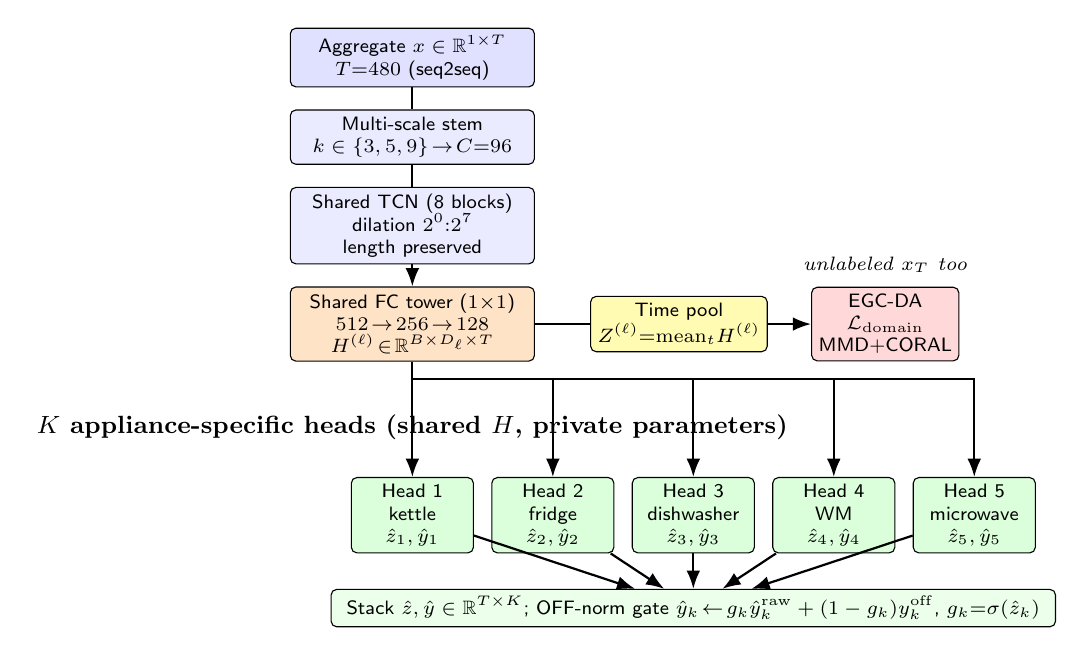
\begin{tikzpicture}[
  font=\scriptsize\sffamily,
  node distance=0.28cm and 0.35cm,
  blk/.style={draw, align=center, rounded corners=2pt, inner sep=2.5pt},
  arr/.style={-{Latex}, thick},
  head/.style={blk, fill=green!14, minimum width=1.55cm, minimum height=0.95cm}
]
% Encoder column
\node[blk, fill=blue!12, minimum width=3.1cm] (in) {Aggregate $x\in\mathbb{R}^{1\times T}$\\$T{=}480$ (seq2seq)};
\node[blk, fill=blue!8, minimum width=3.1cm, below=of in] (stem) {Multi-scale stem\\$k\in\{3,5,9\}\!\rightarrow\!C{=}96$};
\node[blk, fill=blue!8, minimum width=3.1cm, below=of stem] (tcn) {Shared TCN (8 blocks)\\dilation $2^{0}{:}2^{7}$\\length preserved};
\node[blk, fill=orange!22, minimum width=3.1cm, below=of tcn] (fc) {Shared FC tower ($1{\times}1$)\\$512\!\rightarrow\!256\!\rightarrow\!128$\\$H^{(\ell)}\!\in\!\mathbb{R}^{B\times D_\ell\times T}$};
\draw[arr] (in)--(stem)--(tcn)--(fc);

% DA branch
\node[blk, fill=yellow!30, right=0.7cm of fc] (pool) {Time pool\\$Z^{(\ell)}{=}\mathrm{mean}_t H^{(\ell)}$};
\node[blk, fill=red!15, right=0.55cm of pool] (da) {EGC-DA\\$\mathcal{L}_{\mathrm{domain}}$\\MMD+CORAL};
\draw[arr] (fc)--(pool)--(da);
\node[font=\scriptsize\itshape, above=0.05cm of da] {unlabeled $x_T$ too};

% Multi heads
\node[font=\small\bfseries, below=0.55cm of fc] (htag) {$K$ appliance-specific heads (shared $H$, private parameters)};
\node[head, below=0.35cm of htag] (h1) {Head 1\\kettle\\$\hat{z}_1,\hat{y}_1$};
\node[head, right=0.22cm of h1] (h2) {Head 2\\fridge\\$\hat{z}_2,\hat{y}_2$};
\node[head, right=0.22cm of h2] (h3) {Head 3\\dishwasher\\$\hat{z}_3,\hat{y}_3$};
\node[head, right=0.22cm of h3] (h4) {Head 4\\WM\\$\hat{z}_4,\hat{y}_4$};
\node[head, right=0.22cm of h4] (h5) {Head 5\\microwave\\$\hat{z}_5,\hat{y}_5$};
\draw[arr] (fc.south) -- ++(0,-0.22) -| (h1.north);
\draw[arr] (fc.south) -- ++(0,-0.22) -| (h2.north);
\draw[arr] (fc.south) -- ++(0,-0.22) -| (h3.north);
\draw[arr] (fc.south) -- ++(0,-0.22) -| (h4.north);
\draw[arr] (fc.south) -- ++(0,-0.22) -| (h5.north);

\node[blk, fill=green!8, below=0.45cm of h3, minimum width=9.2cm] (out)
  {Stack $\hat{z},\hat{y}\in\mathbb{R}^{T\times K}$;
   OFF-norm gate $\hat{y}_k\!\leftarrow\!g_k\hat{y}^{\mathrm{raw}}_k+(1-g_k)y_k^{\mathrm{off}}$,\ $g_k{=}\sigma(\hat{z}_k)$};
\draw[arr] (h1)--(out); \draw[arr] (h2)--(out); \draw[arr] (h3)--(out);
\draw[arr] (h4)--(out); \draw[arr] (h5)--(out);
\end{tikzpicture}
\caption{MATUDA architecture. A shared stem--TCN--FC encoder produces temporal features for domain alignment (after pooling) and for $K{=}5$ private appliance heads (multi-label state + power). Domain adaptation never requires target appliance labels.}
\label{fig:arch}
\end{figure*}

\subsection{Sequence-to-sequence prediction}
Following length-preserving TCN practice in deep domain adaptation for NILM~\cite{lin2022dda} and multi-appliance full-window decoding~\cite{xiong2023matnilm}, the network observes $T{=}480$ samples and predicts appliance powers and states for \emph{every} timestep in the window.
This differs from sequence-to-point decoding of only the window center~\cite{zhang2018seq2point}.
Sliding-window strides are $240$ for both training and evaluation; overlapping windows are reconstructed by mean aggregation when needed.
Table~\ref{tab:window} lists the windowing contract.

\begin{table}[!t]
\caption{Windowing and supervision.}
\label{tab:window}
\centering
\scriptsize
\begin{tabular}{@{}ll@{}}
\toprule
Item & Setting \\
\midrule
Prediction mode & Sequence-to-sequence (full window) \\
Input / output length $T$ & 480 / 480 samples ($\approx$48\,min at 6\,s) \\
Outputs & $K$ power trajectories + $K$ state-logit trajectories \\
Train / eval stride & 240 / 240 \\
Mains column & \texttt{aggregate} \\
\bottomrule
\end{tabular}
\end{table}

\subsection{Temporal encoder}
A multi-scale 1-D stem with kernels $\{3,5,9\}$ captures short waveform edges; channel outputs are concatenated and projected to $C{=}96$ channels.
Eight dilated causal residual TCN blocks with dilations $2^{0},\ldots,2^{7}$ expand the receptive field while \emph{preserving} length $T$, following Lin \emph{et al.}~\cite{lin2022dda}.
Dropout $0.15$ is applied inside residual blocks.

\subsection{FC adaptation tower and per-appliance heads}
A pointwise ($1{\times}1$) FC tower maps channels through $512\rightarrow 256\rightarrow 128$ with ReLU and dropout, yielding temporal feature maps $H^{(\ell)}\in\mathbb{R}^{B\times D_\ell\times T}$.
For domain adaptation we form
\begin{equation}
Z^{(\ell)}=\mathrm{mean}_{t}\,H^{(\ell)}\in\mathbb{R}^{B\times D_\ell},
\quad \ell=1,2,3,
\label{eq:pool}
\end{equation}
i.e., Lin fc6--fc8 analogues after temporal pooling~\cite{lin2022dda}.
Each of the $K$ appliances then has its own small Conv1d head (local refine $\rightarrow$ state logit + power), reducing competition across loads with very different scales and ON rates.
With soft gating, predicted power is blended toward the appliance OFF level in normalized space,
\begin{equation}
\hat{y}_{k}=g_{k}\,\hat{y}^{\mathrm{raw}}_{k}+(1-g_{k})\,y_{k}^{\mathrm{off}},
\quad
g_{k}=\sigma(\hat{z}_{k}),
\label{eq:gate}
\end{equation}
where $y_{k}^{\mathrm{off}}$ is the z-score of $0$\,W for appliance $k$.
The full model has approximately $0.85$\,M trainable parameters.

%----------------------------------------------------------------------
\subsection{Loss design for multi-appliance multi-label UDA}
\label{sec:loss}
%----------------------------------------------------------------------
Fig.~\ref{fig:loss} summarizes the objective.
Only the source batch contributes supervised multi-task terms; the target batch contributes domain (and optional pseudo-label) terms that do not need $y_T$ or $z_T$.

\begin{figure}[!t]
\centering
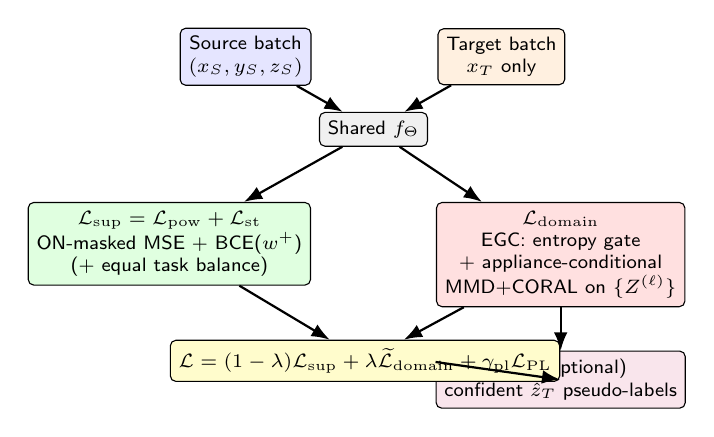
\begin{tikzpicture}[
  font=\scriptsize\sffamily,
  node distance=0.35cm and 0.45cm,
  blk/.style={draw, rounded corners=2pt, align=center, inner sep=3pt},
  arr/.style={-{Latex}, thick}
]
\node[blk, fill=blue!10] (S) {Source batch\\$(x_S,y_S,z_S)$};
\node[blk, fill=orange!12, right=1.6cm of S] (T) {Target batch\\$x_T$ only};
\node[blk, fill=gray!12, below=0.7cm of $(S)!0.5!(T)$] (F) {Shared $f_\Theta$};
\draw[arr] (S)--(F); \draw[arr] (T)--(F);

\node[blk, fill=green!12, below left=0.7cm and 0.1cm of F] (sup)
  {$\mathcal{L}_{\mathrm{sup}}=\mathcal{L}_{\mathrm{pow}}+\mathcal{L}_{\mathrm{st}}$\\
   ON-masked MSE + BCE($w^+$)\\
   (+ equal task balance)};
\node[blk, fill=red!12, below right=0.7cm and 0.1cm of F] (dom)
  {$\mathcal{L}_{\mathrm{domain}}$\\
   EGC: entropy gate\\
   + appliance-conditional\\
   MMD+CORAL on $\{Z^{(\ell)}\}$};
\node[blk, fill=purple!10, below=0.55cm of dom] (pl)
  {$\mathcal{L}_{\mathrm{PL}}$ (optional)\\
   confident $\hat{z}_T$ pseudo-labels};
\draw[arr] (F)--(sup);
\draw[arr] (F)--(dom);
\draw[arr] (dom)--(pl);

\node[blk, fill=yellow!20, below=1.15cm of $(sup)!0.5!(dom)$] (tot)
  {$\mathcal{L}=(1-\lambda)\mathcal{L}_{\mathrm{sup}}+\lambda\widetilde{\mathcal{L}}_{\mathrm{domain}}+\gamma_{\mathrm{pl}}\mathcal{L}_{\mathrm{PL}}$};
\draw[arr] (sup)--(tot);
\draw[arr] (dom)--(tot);
\draw[arr] (pl)--(tot);
\end{tikzpicture}
\caption{Loss composition. Supervised multi-appliance multi-label terms use source labels only; domain and pseudo-label terms use unlabeled target aggregates.}
\label{fig:loss}
\end{figure}

\paragraph{Why the design is layered.}
A single MSE or BCE on a shared head is insufficient here.
Power regression is dominated by high-duty appliances (e.g., fridge), while rare spikes (kettle, microwave) need strong classification gradients.
Domain alignment on raw temporal maps can hurt sparse heads~\cite{muaz2024when}; aligning pooled FC embeddings, then conditioning on predicted multi-label states, is our remedy.
Optional confident target pseudo-labels~\cite{hur2022ssda} further stabilize the multi-label decision boundary after a source-only warmup.

\paragraph{Supervised power term (source).}
Let $m_S=z_S\in\{0,1\}^{T\times K}$ be the multi-label ON mask.
We use ON-masked MSE so OFF timesteps do not dominate the regression:
\begin{equation}
\mathcal{L}_{\mathrm{pow}}
=
\lambda_{y}\,
\frac{\big\|m_S\odot(\hat{y}_S-y_S)\big\|_2^{2}}{\|m_S\|_1+\varepsilon}.
\label{eq:pow}
\end{equation}

\paragraph{Supervised multi-label state term (source).}
States are treated as $K$ simultaneous binary labels over time.
With per-appliance positive weights $w^{+}_{k}=\min(50,\,n_{\mathrm{neg},k}/n_{\mathrm{pos},k})$ estimated on source training only,
\begin{equation}
\mathcal{L}_{\mathrm{st}}^{\mathrm{raw}}
=
\mathrm{BCE}_{\mathrm{logits}}(\hat{z}_S,z_S;w^{+}).
\label{eq:st}
\end{equation}
Because MSE and BCE live on different numeric scales, we apply MultiNILM-style \emph{equal task balance}:
\begin{equation}
\mathcal{L}_{\mathrm{st}}
=
\lambda_{z}\,
\mathcal{L}_{\mathrm{st}}^{\mathrm{raw}}
\cdot
\frac{\mathcal{L}_{\mathrm{pow}}}{\mathcal{L}_{\mathrm{st}}^{\mathrm{raw}}}\Big|_{\mathrm{sg}},
\label{eq:balance}
\end{equation}
so $\lambda_{z}{=}1$ means equal magnitude of power and state contributions.
Then
\begin{equation}
\mathcal{L}_{\mathrm{sup}}=\mathcal{L}_{\mathrm{pow}}+\mathcal{L}_{\mathrm{st}}.
\label{eq:sup}
\end{equation}

\paragraph{Domain term without target labels.}
Source and target windows are passed through the same encoder.
Layer-wise hybrid alignment on pooled FC features~\cite{lin2022dda,sun2016deepcoral} is
\begin{equation}
\mathcal{L}^{(\ell)}
=
\mu\,\mathrm{MMD}^{2}\!\big(Z_S^{(\ell)},Z_T^{(\ell)}\big)
+
(1-\mu)\,\mathcal{L}_{\mathrm{CORAL}}\!\big(Z_S^{(\ell)},Z_T^{(\ell)}\big),
\label{eq:hyb}
\end{equation}
with $\mu{=}0.4$.
Global FC-UDA sums~\eqref{eq:hyb} over $\ell=1,2,3$ (Lin Eq.~12).

\paragraph{EGC-DA for multi-label transfer.}
Uniform alignment can still induce negative transfer among sparse and dense appliances~\cite{muaz2024when}.
EGC-DA (inspired by CDAN+E~\cite{long2018cdan}) adds:
\begin{enumerate}
\item \textbf{Entropy gate.} Sample weight
$w=1-\bar{H}(\sigma(\hat{z}))/\ln 2$ (mean binary entropy over time and the $K$ labels) down-weights uncertain windows before global MMD+CORAL.
\item \textbf{Appliance-conditional alignment.} On the last FC layer, soft-weight embeddings by the time-averaged ON probability of each appliance and average hybrid losses over appliances with sufficient predicted ON mass ($\ge 2.0$) on both domains.
\end{enumerate}
We blend gated-global and conditional terms with equal weight $0.5$ to form $\mathcal{L}_{\mathrm{domain}}$.

\paragraph{Optional target pseudo-labels.}
After source-only warmup, confident target multi-label predictions
($\max(\sigma(\hat{z}_T),1-\sigma(\hat{z}_T))\ge\tau$, default $\tau{=}0.9$)
provide hard pseudo-labels for a BCE term $\mathcal{L}_{\mathrm{PL}}$ with weight $\gamma_{\mathrm{pl}}$ (default $0.3$)~\cite{hur2022ssda}.

\paragraph{Total objective.}
Convex mixing~\cite{lin2022dda} with stop-grad magnitude matching of the domain term yields
\begin{equation}
\begin{aligned}
\mathcal{L}
&=
(1-\lambda)\mathcal{L}_{\mathrm{sup}}
+
\lambda\,\widetilde{\mathcal{L}}_{\mathrm{domain}}
+
\gamma_{\mathrm{pl}}\,\mathcal{L}_{\mathrm{PL}},
\\
\widetilde{\mathcal{L}}_{\mathrm{domain}}
&=
\mathcal{L}_{\mathrm{domain}}\cdot
\frac{\mathcal{L}_{\mathrm{sup}}}{|\mathcal{L}_{\mathrm{domain}}|}\Big|_{\mathrm{sg}}.
\end{aligned}
\label{eq:total}
\end{equation}
Default $\lambda\in\{0.5,0.6\}$.
For the first $N_{\mathrm{warm}}$ epochs (default $30$) we set $\lambda{=}0$ and $\gamma_{\mathrm{pl}}{=}0$ (source-only), then enable DA and pseudo-labeling.
Algorithm~\ref{alg:train} summarizes one post-warmup step.

\begin{table}[!t]
\caption{Fixed z-score normalization constants (hand-set UK-DALE convention; not target/test statistics).}
\label{tab:norm}
\centering
\scriptsize
\begin{tabular}{@{}lcc@{}}
\toprule
Signal & Mean & Std \\
\midrule
Aggregate & 400 & 500 \\
Kettle & 100 & 500 \\
Fridge & 50 & 50 \\
Dishwasher & 700 & 1000 \\
Washing machine & 400 & 700 \\
Microwave & 60 & 300 \\
\bottomrule
\end{tabular}
\end{table}

\begin{algorithm}[!t]
\caption{One MATUDA training step (unsupervised DA; after warmup)}
\label{alg:train}
\begin{algorithmic}[1]
\REQUIRE Source batch $(x_S,y_S,z_S)$, target batch $x_T$, weights $\Theta$, $\lambda$, $\gamma_{\mathrm{pl}}$
\STATE $(\hat{y}_S,\hat{z}_S,\{Z_S^{(\ell)}\})\leftarrow f_\Theta(x_S)$
\STATE $(\hat{y}_T,\hat{z}_T,\{Z_T^{(\ell)}\})\leftarrow f_\Theta(x_T)$ \COMMENT{labels unused}
\STATE Compute $\mathcal{L}_{\mathrm{pow}}$, $\mathcal{L}_{\mathrm{st}}$, $\mathcal{L}_{\mathrm{sup}}$ on source using~\eqref{eq:pow}--\eqref{eq:sup}
\STATE Compute $\mathcal{L}_{\mathrm{domain}}$ on $\{Z_S^{(\ell)},Z_T^{(\ell)}\}$ (Global FC-UDA or EGC-DA)
\STATE Optionally compute confident-target $\mathcal{L}_{\mathrm{PL}}$ from $\hat{z}_T$
\STATE Form $\mathcal{L}$ by~\eqref{eq:total}; update $\Theta$ by AdamW
\end{algorithmic}
\end{algorithm}

Aggregates and powers are z-score normalized with fixed hand-set UK-DALE constants (Table~\ref{tab:norm}), taken from a common multi-appliance NILM preprocessing convention and \emph{not} recomputed on House~2 or on the held-out test segment; reported metrics use denormalized watts.

%======================================================================
\section{Experimental Setup}
%======================================================================
\subsection{Dataset and transfer scenario}
We use low-frequency UK-DALE active power~\cite{kelly2015ukdale}.
Appliances ($K{=}5$): kettle, fridge, dishwasher, washing machine, microwave---the intersection on Houses~1, 2, and~5.
Houses~3 and~4 lack several of these submeters and are not used as labeled sources for this set.

Processed CSVs provide aligned aggregate, appliance power, and on/off columns with a house index.
On/off labels in the CSV follow fixed power thresholds (W): kettle~$40$, fridge~$50$, dishwasher~$30$, washing machine~$30$, microwave~$100$.
Missing samples are excluded during CSV construction; windows require a complete contiguous length-$T$ aggregate segment.

\textbf{Train/val:} Houses~1+5 labeled windows.
\textbf{Target adaptation:} House~2 aggregates only, using the first $70\%$ of the House~2 timeline (unlabeled).
\textbf{Target test:} the remaining $30\%$ of House~2 (labels used solely for metrics).
Adaptation and evaluation windows therefore do not share timesteps; overlapping sliding windows within each segment use stride $240$.
Aggregate mean power differs strongly across domains (source $\approx$1089\,W vs.\ House~2 $\approx$311\,W), confirming a non-trivial shift.

\subsection{Compared methods (same backbone)}
All methods share the MATUDA encoder and heads; only the domain term changes.
\begin{itemize}
\item \textbf{Source-Only:} $\lambda{=}0$ (no target adaptation).
\item \textbf{Global FC-UDA:} multi-layer FC MMD+CORAL~\eqref{eq:hyb}.
\item \textbf{MATUDA:} EGC-DA on top of the same FC hybrid loss.
\end{itemize}
Ablations (MMD-only, CORAL-only, EGC without entropy, EGC without conditional alignment) and additional house splits are part of the journal evaluation plan; Tables~\ref{tab:main}--\ref{tab:perapp} currently report a single-seed pilot under an earlier protocol and will be replaced by mean$\pm$std results on the chronological split.

\subsection{Implementation details}
Table~\ref{tab:impl} lists hyperparameters.
Model selection uses source validation MAE; House~2 is never used for checkpoint choice.
Training runs on an NVIDIA RTX~4090 (PyTorch 2.6, CUDA 12.4).

\begin{table}[!t]
\caption{Implementation details (paper configuration).}
\label{tab:impl}
\centering
\scriptsize
\begin{tabular}{@{}ll@{}}
\toprule
Item & Value \\
\midrule
Optimizer & AdamW, lr $10^{-3}$, weight decay $10^{-4}$ \\
Schedule & ReduceLROnPlateau on source val MAE$-$F1 \\
Batch size & 32 \\
$\lambda$ (DA) / source-only warmup & $0.5$--$0.6$ / $30$ epochs (EGC+PL) \\
$\mu$ (MMD vs.\ CORAL) & 0.4 \\
Pseudo-label weight / confidence & $0.3$ / $0.9$ (optional) \\
Conditional ON-mass threshold & $2.0$ \\
Positive-weight cap & $50$ \\
Gradient clip & 5.0 \\
Seeds (journal runs) & $\{2024,2025,2026\}$ \\
\bottomrule
\end{tabular}
\end{table}

\subsection{Metrics}
\textbf{State detection:} per-appliance precision, recall, and F1 (threshold $0.5$ on $\sigma(\hat{z})$), plus macro-F1.
\textbf{Power estimation:} MAE and relative energy error SAE after denormalization to watts.
We also report $\Delta$F1 versus Source-Only.

%======================================================================
\section{Results and Discussion}
%======================================================================
\subsection{Cross-building performance (preliminary)}
Table~\ref{tab:main} reports House~2 metrics for checkpoints selected by source validation MAE.
These numbers are from a single-seed pilot in which House~2 aggregates were used for both adaptation and evaluation; they are retained only to illustrate the qualitative pattern and will be superseded by multi-seed results on the chronological $70\%$/$30\%$ split described above.

All three methods fit the source domain well (validation macro-F1 $\approx 0.82$--$0.84$).
On House~2, Source-Only macro-F1 collapses to $0.087$: multi-appliance multi-label decoding does not transfer automatically.
Global FC-UDA raises F1 only to $0.143$ while increasing MAE from $29.3$\,W to $49.6$\,W---evidence of negative transfer on regression heads under uniform alignment~\cite{muaz2024when}.
MATUDA reaches macro-F1 $0.469$ ($+0.382$ absolute vs.\ Source-Only) with MAE $32.2$\,W, close to Source-Only.
However, SAE rises from $1.21$ (Source-Only) to $2.32$ (MATUDA): energy estimation is worse even when detection F1 improves.
We therefore do not claim that adaptation preserves energy accuracy; the practical trade-off is F1 gains versus SAE degradation.

\begin{table}[!t]
\caption{UK-DALE Houses 1+5 $\rightarrow$ House 2 (unsupervised). Preliminary single-seed pilot (overlapping adapt/eval protocol; to be replaced). Selection by source validation MAE.}
\label{tab:main}
\centering
\scriptsize
\begin{tabular}{@{}lcccc@{}}
\toprule
Method & Macro-F1 $\uparrow$ & MAE (W) $\downarrow$ & SAE $\downarrow$ & $\Delta$F1 \\
\midrule
Source-Only & 0.087 & \textbf{29.3} & \textbf{1.21} & --- \\
Global FC-UDA & 0.143 & 49.6 & 2.91 & $+0.056$ \\
\textbf{MATUDA (EGC-DA)} & \textbf{0.469} & 32.2 & 2.32 & $\mathbf{+0.382}$ \\
\bottomrule
\end{tabular}
\end{table}

Table~\ref{tab:perapp} breaks down House~2 F1.
MATUDA improves kettle, fridge, washing machine, and microwave substantially.
Dishwasher remains at zero F1 for all methods.
House~2 dishwasher ON events are extremely sparse relative to fridge cycling; under severe class imbalance, both source-only and adapted models suppress the rare head.
We treat dishwasher as an open failure mode and plan event-count, duration, and confusion analysis in the journal revision.

\begin{table}[!t]
\caption{Per-appliance House~2 F1 (same preliminary checkpoints as Table~\ref{tab:main}).}
\label{tab:perapp}
\centering
\scriptsize
\begin{tabular}{@{}lccccc@{}}
\toprule
Method & Kettle & Fridge & DW & WM & MW \\
\midrule
Source-Only & 0.12 & 0.27 & 0.00 & 0.00 & 0.04 \\
Global FC-UDA & 0.17 & 0.45 & 0.00 & 0.00 & 0.10 \\
\textbf{MATUDA} & \textbf{0.78} & \textbf{0.76} & 0.00 & \textbf{0.52} & \textbf{0.28} \\
\bottomrule
\end{tabular}
\end{table}

\subsection{Training dynamics and qualitative power traces}
Figure~\ref{fig:train_compare} plots House~2 macro-F1 and MAE over epochs for the three methods under the same backbone.
Source-Only and Global FC-UDA remain weak on House~2 F1 throughout training, whereas MATUDA shows a late rise in F1 together with a reduction in MAE.
This confirms that the tabulated gains are not a single-checkpoint artifact, but also that target performance is unstable early in training.

\begin{figure*}[!t]
\centering
\includegraphics[width=0.95\textwidth]{figures/train_compare_h2_f1_mae.png}
\caption{House~2 macro-F1 and MAE during training for Source-Only, Global FC-UDA, and MATUDA (same backbone; preliminary pilot).}
\label{fig:train_compare}
\end{figure*}

Figure~\ref{fig:power_grid} compares House~2 appliance power predictions for Source-Only versus MATUDA on a contiguous test segment.
Source-Only largely collapses to near-zero predictions for kettle, dishwasher, and washing machine.
MATUDA recovers some event structure, but still misses dishwasher activations and frequently assigns dishwasher energy to washing-machine / microwave heads---a qualitative explanation for dishwasher F1~$=$~$0$ and elevated SAE.

\begin{figure*}[!t]
\centering
\includegraphics[width=0.48\textwidth]{figures/h2_power_grid_source_only.png}
\hfill
\includegraphics[width=0.48\textwidth]{figures/h2_power_grid_matuda.png}
\caption{House~2 power traces (true vs.\ predicted). Left: Source-Only collapse. Right: MATUDA recovers some events but confuses dishwasher with other high-power loads.}
\label{fig:power_grid}
\end{figure*}

Figure~\ref{fig:train_matuda} shows MATUDA supervised/domain losses and source-validation versus House~2 metrics; source validation F1 remains high while House~2 F1 is much lower, confirming domain shift rather than source underfitting.

\begin{figure}[!t]
\centering
\includegraphics[width=\columnwidth]{figures/train_curves_matuda_s2_m0_egc.png}
\caption{MATUDA training curves: train loss, source-validation F1/MAE, and House~2 F1/MAE (green dashed line: checkpoint selected by source validation MAE).}
\label{fig:train_matuda}
\end{figure}

\subsection{Discussion}
\paragraph{Why Source-Only can have low MAE but poor F1.}
For sparse appliances, predicting near-zero power most of the time yields moderate MAE while missing ON events (F1$\approx 0$).
MATUDA recovers ON detection; per-appliance MAE can improve for kettle/fridge but may increase for event-driven loads when activations are imperfect, so mean MAE stays near Source-Only while SAE may rise.

\paragraph{Why Global FC-UDA is insufficient.}
Forcing one shared embedding to match target aggregates helps states only slightly and harms power---exactly the multi-task negative-transfer regime that motivates EGC-DA.

\paragraph{Scope of claims.}
We claim that unsupervised multi-appliance multi-label cross-building transfer is a well-posed problem and that FC-layer EGC-DA is a promising adaptation mechanism on UK-DALE H1+H5$\rightarrow$H2.
We do not claim dishwasher is solved, that SAE is preserved, that one house split generalizes to all UK-DALE transfers, or that cross-dataset transfer is complete.

\subsection{Limitations and revision plan}
The present manuscript remains below top-tier journal evidence standards until the following are completed: (i)~multi-seed mean$\pm$std on the chronological House~2 split; (ii)~component ablations of EGC-DA; (iii)~additional UK-DALE house directions; (iv)~stronger baselines (MMD/CORAL-only, adversarial DA, supervised target fine-tuning upper bound); (v)~cross-dataset UK-DALE$\leftrightarrow$REDD/REFIT; and (vi)~per-appliance precision/recall/MAE/SAE with dishwasher event analysis.

%======================================================================
\section{Conclusion}
%======================================================================
This paper presented MATUDA for unsupervised transfer of joint multi-label and multi-appliance NILM: a sequence-to-sequence TCN with a shared pointwise FC adaptation tower, $K$ appliance-specific heads, and EGC-DA (optionally with confident target pseudo-labels).
Under a UK-DALE cross-building scenario, preliminary results show large macro-F1 gains from EGC-DA relative to Source-Only and Global FC-UDA, together with a clear SAE degradation that must be reported honestly.
Ongoing work replaces the pilot tables with multi-seed chronological-split evaluation, ablations, multi-house and cross-dataset protocols, and deeper analysis of sparse loads such as the dishwasher.

\begin{thebibliography}{00}
\bibitem{hart1992nilm} G.~W. Hart, ``Nonintrusive appliance load monitoring,'' \emph{Proc. IEEE}, vol.~80, no.~12, pp.~1870--1891, 1992.
\bibitem{kelly2015ukdale} J.~Kelly and W.~Knottenbelt, ``The UK-DALE dataset, domestic appliance-level electricity demand and whole-house demand from five UK homes,'' \emph{Sci. Data}, vol.~2, Art.~150007, 2015.
\bibitem{kelly2015neural} J.~Kelly and W.~Knottenbelt, ``Neural NILM: Deep neural networks applied to energy disaggregation,'' in \emph{Proc. BuildSys}, 2015, pp.~55--64.
\bibitem{zhang2018seq2point} C.~Zhang, M.~Zhong, Z.~Wang, N.~Goddard, and C.~Sutton, ``Sequence-to-point learning for non-intrusive load monitoring,'' in \emph{Proc. AAAI}, 2018.
\bibitem{faustine2020unet} A.~Faustine, L.~Pereira, and C.~Klemenjak, ``UNet-NILM: A deep neural network for multi-appliance NILM,'' in \emph{Proc. NILM Workshop}, 2020.
\bibitem{xiong2023matnilm} Z.~Xiong \emph{et al.}, ``MATNilm: Multi-appliance-task non-intrusive load monitoring with limited labeled data,'' \emph{IEEE Trans. Ind. Informat.}, 2023.
\bibitem{liu2022uda} Y.~Liu, J.~Wang, and J.~Deng, ``Unsupervised domain adaptation for non-intrusive load monitoring,'' \emph{IEEE Trans. Ind. Informat.}, 2022.
\bibitem{lin2022dda} J.~Lin, J.~Ma, J.~Zhu, and H.~Liang, ``Deep domain adaptation for non-intrusive load monitoring based on a knowledge transfer learning network,'' \emph{IEEE Trans. Smart Grid}, vol.~13, no.~1, pp.~280--292, Jan.~2022.
\bibitem{xiong2026ahda} Hierarchical distribution alignment for NILM transfer, \emph{Electronics}, 2026.
\bibitem{lu2026edge} T.~Lu \emph{et al.}, ``Unsupervised lightweight transfer learning for NILM,'' \emph{IEEE Trans. Smart Grid}, 2026.
\bibitem{dincecco2020transfer} M.~D'Incecco, S.~Squartini, and M.~Zhong, ``Transfer learning for non-intrusive load monitoring,'' \emph{IEEE Trans. Smart Grid}, vol.~11, no.~2, pp.~1419--1429, 2020.
\bibitem{sun2025transfer} Y.~Sun \emph{et al.}, ``Transfer learning for multi-appliance-task NILM,'' \emph{IEEE Trans. Instrum. Meas.}, 2025.
\bibitem{li2023multiobjective} D.~Li \emph{et al.}, ``Transfer learning for multi-objective non-intrusive load monitoring in smart grid,'' \emph{Appl. Energy}, 2023.
\bibitem{hur2022ssda} C.~Hur \emph{et al.}, ``Semi-supervised domain adaptation for multi-label NILM,'' \emph{Sensors}, 2022.
\bibitem{tanoni2023weak} G.~Tanoni, E.~Principi, and S.~Squartini, ``Multilabel appliance classification with weakly labeled data for non-intrusive load monitoring,'' \emph{IEEE Trans. Smart Grid}, 2023.
\bibitem{muaz2024when} M.~Muaz \emph{et al.}, ``NILM domain adaptation: When does it work?'' in \emph{Proc. ICSCC}, 2024.
\bibitem{sun2016deepcoral} B.~Sun and K.~Saenko, ``Deep CORAL: Correlation alignment for deep domain adaptation,'' in \emph{ECCV Workshops}, 2016.
\bibitem{long2015dan} M.~Long, Y.~Cao, J.~Wang, and M.~Jordan, ``Learning transferable features with deep adaptation networks,'' in \emph{Proc. ICML}, 2015.
\bibitem{long2018cdan} M.~Long, Z.~Cao, J.~Wang, and M.~I. Jordan, ``Conditional adversarial domain adaptation,'' in \emph{Proc. NeurIPS}, 2018.
\end{thebibliography}

\end{document}
